\section*{Digital Timing}

We can perform a digital timing that reconstructs all the analog chain using software. In order to do so we need the signal waveforms provided by the DT5751 CAEN digitizer\footnote{with a sampling rate of 1 GS/s}.
The digitized waveform then is manipulated in order to obtain a bipolar signal (Fig.\ref{Fig: digital waveform manipulations}).
\begin{figure}[h!]
\centering
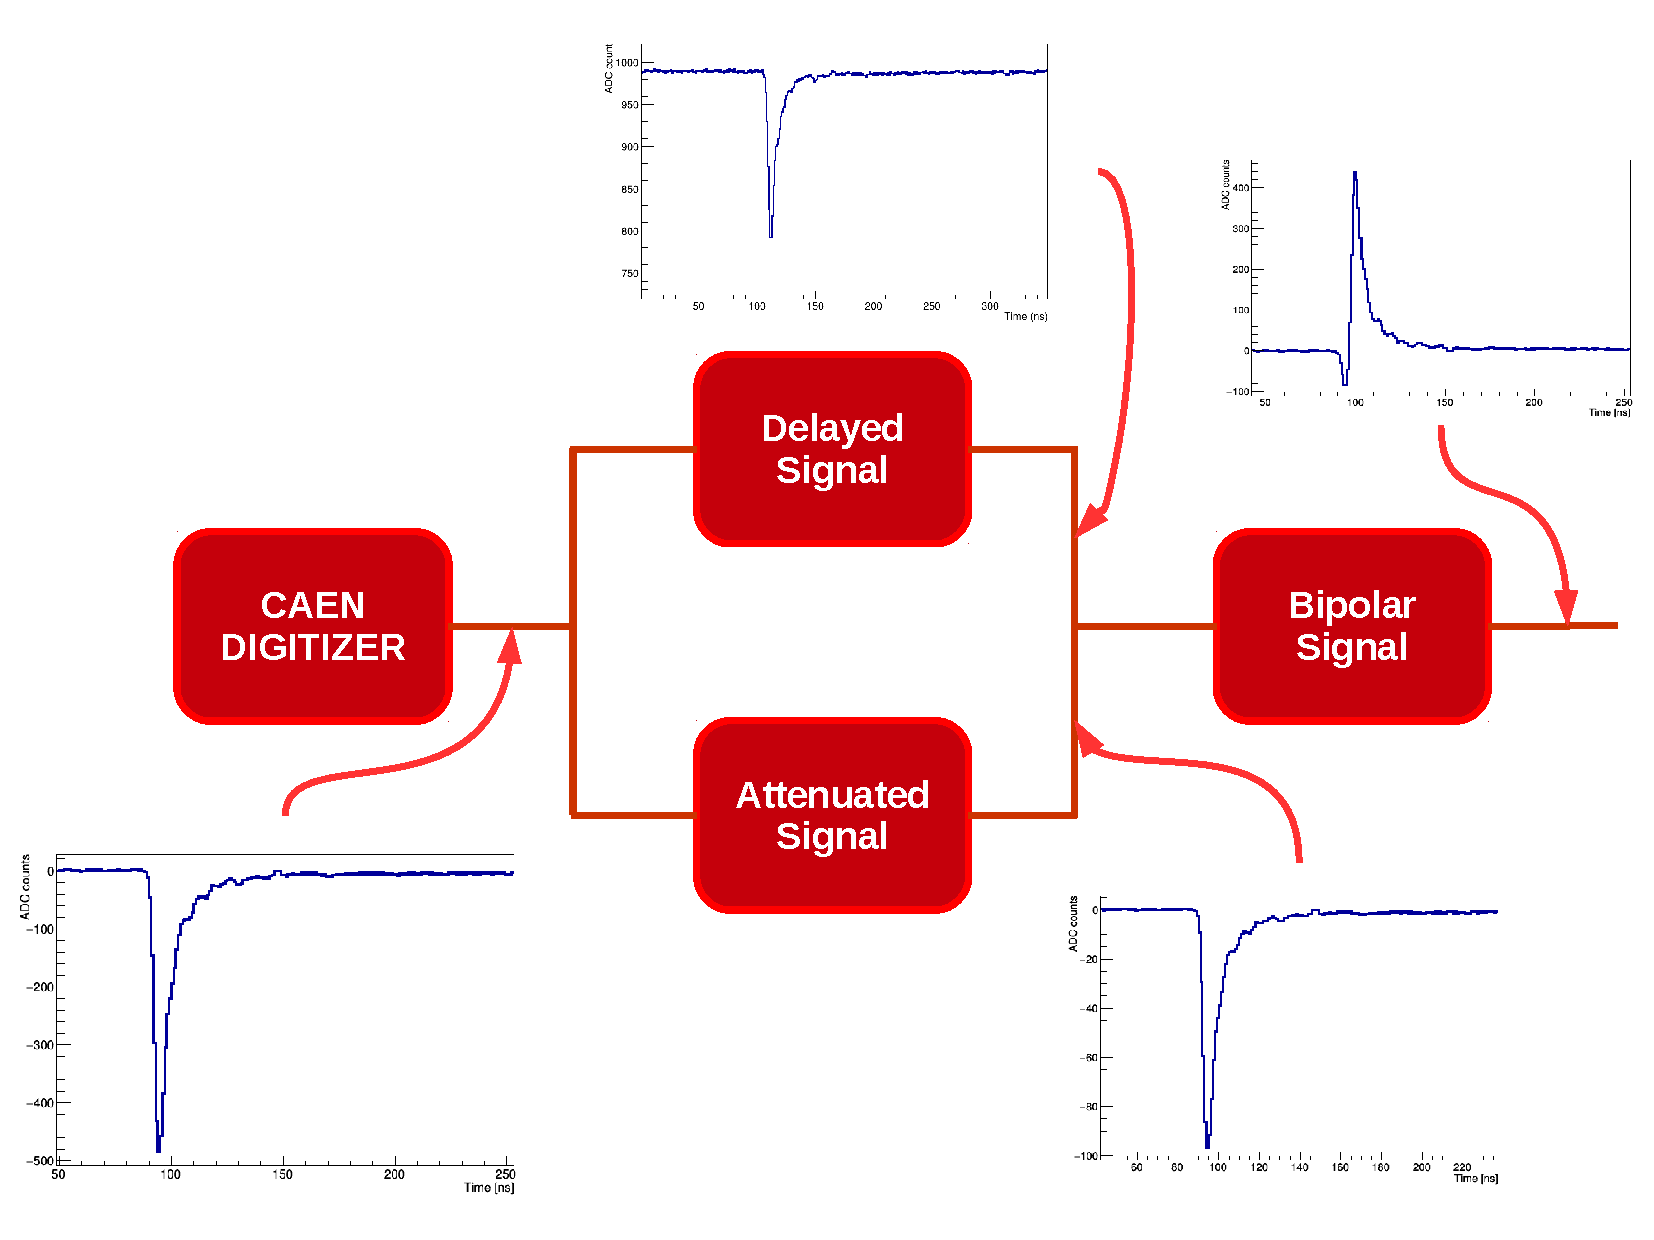
\includegraphics[width=\textwidth]{digital_waveform}
\caption{Digital waveforms manipulations used to get the bipolar signal}
\label{Fig: digital waveform manipulations}
\end{figure}
Then troughtout an algorithms we have to find the zero of the signal that is the time that we associate to the event.

\medskip
descrizione dell'algoritmo e del fit c2 etc etc
\medskip

\noindent The bipolar signal shape depends on two parameter that we need to tune in order to optimize the time resolution:
\begin{itemize}
\item Fraction
\item Delay
\end{itemize}


